\documentclass{ximera}

 

\usepackage{epsfig}

\graphicspath{
  {./}
  {figures/}
}

\usepackage{morewrites}
\makeatletter
\newcommand\subfile[1]{%
\renewcommand{\input}[1]{}%
\begingroup\skip@preamble\otherinput{#1}\endgroup\par\vspace{\topsep}
\let\input\otherinput}
\makeatother

\newcommand{\includeexercises}{\directlua{dofile("/home/jim/linearAlgebra/laode/exercises.lua")}}

%\newcounter{ccounter}
%\setcounter{ccounter}{1}
%\newcommand{\Chapter}[1]{\setcounter{chapter}{\arabic{ccounter}}\chapter{#1}\addtocounter{ccounter}{1}}

%\newcommand{\section}[1]{\section{#1}\setcounter{thm}{0}\setcounter{equation}{0}}

%\renewcommand{\theequation}{\arabic{chapter}.\arabic{section}.\arabic{equation}}
%\renewcommand{\thefigure}{\arabic{chapter}.\arabic{figure}}
%\renewcommand{\thetable}{\arabic{chapter}.\arabic{table}}

%\newcommand{\Sec}[2]{\section{#1}\markright{\arabic{ccounter}.\arabic{section}.#2}\setcounter{equation}{0}\setcounter{thm}{0}\setcounter{figure}{0}}

\newcommand{\Sec}[2]{\section{#1}}

\setcounter{secnumdepth}{2}
%\setcounter{secnumdepth}{1} 

%\newcounter{THM}
%\renewcommand{\theTHM}{\arabic{chapter}.\arabic{section}}

\newcommand{\trademark}{{R\!\!\!\!\!\bigcirc}}
%\newtheorem{exercise}{}

\newcommand{\dfield}{{\sf dfield9}}
\newcommand{\pplane}{{\sf pplane9}}

\newcommand{\EXER}{\section*{Exercises}}%\vspace*{0.2in}\hrule\small\setcounter{exercise}{0}}
\newcommand{\CEXER}{}%\vspace{0.08in}\begin{center}Computer Exercises\end{center}}
\newcommand{\TEXER}{} %\vspace{0.08in}\begin{center}Hand Exercises\end{center}}
\newcommand{\AEXER}{} %\vspace{0.08in}\begin{center}Hand Exercises\end{center}}

% BADBAD: \newcommand{\Bbb}{\bf}

\newcommand{\R}{\mbox{$\Bbb{R}$}}
\newcommand{\C}{\mbox{$\Bbb{C}$}}
\newcommand{\Z}{\mbox{$\Bbb{Z}$}}
\newcommand{\N}{\mbox{$\Bbb{N}$}}
\newcommand{\D}{\mbox{{\bf D}}}
\usepackage{amssymb}
%\newcommand{\qed}{\hfill\mbox{\raggedright$\square$} \vspace{1ex}}
%\newcommand{\proof}{\noindent {\bf Proof:} \hspace{0.1in}}

\newcommand{\setmin}{\;\mbox{--}\;}
\newcommand{\Matlab}{{M\small{AT\-LAB}} }
\newcommand{\Matlabp}{{M\small{AT\-LAB}}}
\newcommand{\computer}{\Matlab Instructions}
\newcommand{\half}{\mbox{$\frac{1}{2}$}}
\newcommand{\compose}{\raisebox{.15ex}{\mbox{{\scriptsize$\circ$}}}}
\newcommand{\AND}{\quad\mbox{and}\quad}
\newcommand{\vect}[2]{\left(\begin{array}{c} #1_1 \\ \vdots \\
 #1_{#2}\end{array}\right)}
\newcommand{\mattwo}[4]{\left(\begin{array}{rr} #1 & #2\\ #3
&#4\end{array}\right)}
\newcommand{\mattwoc}[4]{\left(\begin{array}{cc} #1 & #2\\ #3
&#4\end{array}\right)}
\newcommand{\vectwo}[2]{\left(\begin{array}{r} #1 \\ #2\end{array}\right)}
\newcommand{\vectwoc}[2]{\left(\begin{array}{c} #1 \\ #2\end{array}\right)}

\newcommand{\ignore}[1]{}


\newcommand{\inv}{^{-1}}
\newcommand{\CC}{{\cal C}}
\newcommand{\CCone}{\CC^1}
\newcommand{\Span}{{\rm span}}
\newcommand{\rank}{{\rm rank}}
\newcommand{\trace}{{\rm tr}}
\newcommand{\RE}{{\rm Re}}
\newcommand{\IM}{{\rm Im}}
\newcommand{\nulls}{{\rm null\;space}}

\newcommand{\dps}{\displaystyle}
\newcommand{\arraystart}{\renewcommand{\arraystretch}{1.8}}
\newcommand{\arrayfinish}{\renewcommand{\arraystretch}{1.2}}
\newcommand{\Start}[1]{\vspace{0.08in}\noindent {\bf Section~\ref{#1}}}
\newcommand{\exer}[1]{\noindent {\bf \ref{#1}}}
\newcommand{\ans}{}
\newcommand{\matthree}[9]{\left(\begin{array}{rrr} #1 & #2 & #3 \\ #4 & #5 & #6
\\ #7 & #8 & #9\end{array}\right)}
\newcommand{\cvectwo}[2]{\left(\begin{array}{c} #1 \\ #2\end{array}\right)}
\newcommand{\cmatthree}[9]{\left(\begin{array}{ccc} #1 & #2 & #3 \\ #4 & #5 &
#6 \\ #7 & #8 & #9\end{array}\right)}
\newcommand{\vecthree}[3]{\left(\begin{array}{r} #1 \\ #2 \\
#3\end{array}\right)}
\newcommand{\cvecthree}[3]{\left(\begin{array}{c} #1 \\ #2 \\
#3\end{array}\right)}
\newcommand{\cmattwo}[4]{\left(\begin{array}{cc} #1 & #2\\ #3
&#4\end{array}\right)}

\newcommand{\Matrix}[1]{\ensuremath{\left(\begin{array}{rrrrrrrrrrrrrrrrrr} #1 \end{array}\right)}}

\newcommand{\Matrixc}[1]{\ensuremath{\left(\begin{array}{cccccccccccc} #1 \end{array}\right)}}



\renewcommand{\labelenumi}{\theenumi)}
\newenvironment{enumeratea}%
{\begingroup
 \renewcommand{\theenumi}{\alph{enumi}}
 \renewcommand{\labelenumi}{(\theenumi)}
 \begin{enumerate}}
 {\end{enumerate}\endgroup}



\newcounter{help}
\renewcommand{\thehelp}{\thesection.\arabic{equation}}

%\newenvironment{equation*}%
%{\renewcommand\endequation{\eqno (\theequation)* $$}%
%   \begin{equation}}%
%   {\end{equation}\renewcommand\endequation{\eqno \@eqnnum
%$$\global\@ignoretrue}}

%\input{psfig.tex}

\author{Martin Golubitsky and Michael Dellnitz}

%\newenvironment{matlabEquation}%
%{\renewcommand\endequation{\eqno (\theequation*) $$}%
%   \begin{equation}}%
%   {\end{equation}\renewcommand\endequation{\eqno \@eqnnum
% $$\global\@ignoretrue}}

\newcommand{\soln}{\textbf{Solution:} }
\newcommand{\exercap}[1]{\centerline{Figure~\ref{#1}}}
\newcommand{\exercaptwo}[1]{\centerline{Figure~\ref{#1}a\hspace{2.1in}
Figure~\ref{#1}b}}
\newcommand{\exercapthree}[1]{\centerline{Figure~\ref{#1}a\hspace{1.2in}
Figure~\ref{#1}b\hspace{1.2in}Figure~\ref{#1}c}}
\newcommand{\para}{\hspace{0.4in}}

\renewenvironment{solution}{\suppress}{\endsuppress}

\ifxake
\newenvironment{matlabEquation}{\begin{equation}}{\end{equation}}
\else
\newenvironment{matlabEquation}%
{\let\oldtheequation\theequation\renewcommand{\theequation}{\oldtheequation*}\begin{equation}}%
  {\end{equation}\let\theequation\oldtheequation}
\fi

\makeatother


\title{Periodic Forcing and Resonance}

\begin{document}
\begin{abstract}
\end{abstract}
\maketitle


\label{S:resonance}

\subsection*{Periodic Forcing}

A linear second order differential equation is {\em periodically forced\/} 
\index{forcing!periodic} if it has the form
\[
\ddot{x} + b\dot{x} + ax = g(t),
\]
where $g(t)$ is periodic in time; that is, $g(t+T) = g(t)$ for some
period $T$.  The simplest kind of forcing is {\em sinusoidal\/} forcing,
\index{forcing!sinusoidal}
that is, $g(t)=\sin(\omega t+ t_0)$ where $\frac{\omega}{2\pi}$ is the 
{\em forcing frequency\/}\index{frequency!forcing} and $t_0$ is a 
{\em phase\/}\index{phase}.  We simplify 
the discussion by choosing the phase $t_0$ so that $g(t)=\cos(\omega t)$ 
and $\omega>0$.

Suppose, in addition, that the homogeneous equation itself has periodic 
solutions\index{periodic solution} with 
{\em internal frequency\/}\index{frequency!internal} 
$\frac{\tau}{2\pi}$.  Such a 
differential equation is $\ddot{x}+\tau^2x=0$; by rescaling time we 
can assume that $\tau=1$.   Thus, the homogeneous equation is 
\[
\ddot x + x = 0,
\]
and the forced equation is
\begin{equation} \label{eq:uspf}
\ddot x + x = \cos(\omega t),
\end{equation}
where $\omega>0$.

We focus on three features of solutions to this equation.
\begin{itemize}
\item[(a)]	Generally, solutions to \Ref{eq:uspf} are quasiperiodic 
\index{motion!quasiperiodic}
having two frequencies\index{frequency} --- just like the torus 
solutions mentioned in Section~\ref{S:NLD}.
\item[(b)]	When the forcing frequency is near the internal frequency, the
solution has beats.
\item[(c)] 	{\em Resonance\/}\index{resonance} occurs when the 
forcing frequency equals the internal frequency.  
\end{itemize}

\subsubsection*{The Periodically Forced Undamped Spring}
\index{spring!undamped}

One of the simplest examples of a model differential equation with both a
forcing frequency and an internal frequency is the periodically forced 
\index{forcing!periodic} undamped spring.

The motion of a forced undamped spring is described by the spring equation 
given in Chapter~\ref{Chap:Planar}, \Ref{e:springeq} with $\mu = 0$.
To simplify the computations, we set the mass to be $m=1$ and suppose that 
the spring constant is $\kappa=1$.  Then, with periodic forcing 
$g(t)=\cos(\omega t)$, we obtain the differential equation \Ref{eq:uspf}.

\subsection*{Closed Form Solutions to \protect{\Ref{eq:uspf}} by Undetermined 
Coefficients}\index{closed form solution}\index{undetermined coefficients}

We can apply the method of undetermined coefficients to solve \Ref{eq:uspf}, 
but there are two cases: $\omega=1$ and $\omega\neq 1$. 

\subsubsection*{The Case $\omega\not= 1$}  

We use undetermined coefficients to find a particular solution to the 
inhomogeneous equation \Ref{eq:uspf}.  The forcing term $\cos(\omega t)$ is 
a solution to the differential equation 
\begin{equation}  \label{E:omega}
\ddot{y} + \omega^2y = 0.
\end{equation}
Thus the annihilator\index{annihilator} 
of $\cos(\omega t)$ is $q(D)=D^2+\omega^2$.  The 
eigenvalues of the homogeneous equation associated to \Ref{eq:uspf} are 
$\pm i$ and the eigenvalues of $q(\lambda)$ are $\pm\omega i$.  Thus when 
$\omega\neq 1$ we can use undetermined coefficients by choosing the general 
solution to \Ref{E:omega} as the trial space\index{trial!space} 
for \Ref{eq:uspf}.  So we set
\[
y(t) = c_1\cos(\omega t) + c_2\sin(\omega t).
\]
Next, substitute $y$ into \Ref{eq:uspf}, obtaining
\[
(1-\omega ^2)(c_1\cos(\omega t) + c_2\sin(\omega t)) = \cos(\omega t).
\]
This equality holds when 
\[
c_1 = \frac{1}{1-\omega ^2} \AND c_2=0.
\]
Since the general solution\index{general solution} of the 
homogeneous\index{homogeneous} equation associated 
to \Ref{eq:uspf} is
\[
\alpha \cos(t)+\beta\sin(t),
\]
the general solution to \Ref{eq:uspf} is
\[
x(t) =\frac{1}{1-\omega ^2}\cos(\omega t) + \alpha\cos(t) + \beta\sin(t),
\]
when $\omega \neq 1$. 

\subsubsection*{The Case $\omega= 1$}

When $\omega= 1$ the roots of $p(\lambda)$ and $q(\lambda)$ both equal 
$\pm i$.  Thus, to use undetermined coefficients, we must first find the 
general solution to 
\[
p(D)q(D)x = 0.
\]
This solution is 
\[
x(t) = \alpha_1\cos t + \alpha_2\sin t + c_1t\cos t + c_2t\sin t.
\]
On setting the solutions to the homogeneous equation associated to 
\Ref{eq:uspf} to zero (that is, on setting $\alpha_1=\alpha_2=0$), we 
find that the trial space for \Ref{eq:uspf} is:
\[
y(t) = c_1t\cos t + c_2t\sin t.
\]
Substituting $y(t)$ into \Ref{eq:uspf} yields:
\[
\ddot{y} + y \equiv -2c_1\sin t + 2c_2\cos t = \cos t.
\]
Therefore, $c_1=0$ and $c_2=\frac{1}{2}$, and a particular solution of 
\Ref{eq:uspf} is 
\[
x_p(t) = \frac{1}{2}t\sin t.
\]
The general solution can be written as
\[
x(t) = \frac{1}{2}t\sin t+\alpha\cos t+\beta\sin t.
\]

To summarize: the general closed form solution to \Ref{eq:uspf} is
\begin{equation}  \label{eq:uspfsoln}
x(t) = \alpha\cos t+\beta\sin t + \left\{\begin{array}{lr}
\frac{1}{1-\omega ^2}\cos(\omega t)  & 0<\omega\neq 1\\  
\frac{1}{2}t\sin t & \omega=1 \end{array}\right.\end{equation}

\subsection*{Types of Solutions to \Ref{eq:uspf}}

We use the closed form solution \Ref{eq:uspfsoln} to \Ref{eq:uspf} to
identify three different types of solutions: quasiperiodic two-frequency 
motion, beats, and resonance.

\subsubsection*{Quasiperiodic Two Frequency Motion}
\index{motion!two frequency}

In our discussion we now specify initial conditions.  In particular, the 
solution to \Ref{eq:uspf} with initial conditions $x(0)=1$ and 
$\dot{x}(0)=0$ is:
\arraystart
\begin{equation}  \label{e:x(t)reson}
x(t) = \cos t + \left\{\begin{array}{ll}
\frac{1}{1-\omega ^2}(\cos(\omega t)-\cos t) & \omega \neq 1 \\
\frac{1}{2}t\sin t & \omega=1  \end{array}\right.
\end{equation}
\arrayfinish
In particular, when $\omega\neq 1$, the solution \Ref{e:x(t)reson} is
just a linear combination of two periodic 
functions\index{linear!combination!of periodic functions} with different 
frequencies\index{frequency}:
\begin{equation} \label{e:x(t)reson2}
x(t) = -\frac{\omega^2}{1-\omega ^2} \cos t + \frac{1}{1-\omega ^2}\cos(\omega t).
\end{equation}
In this way it is straightforward to see that the motion is 
quasiperiodic\index{motion!quasiperiodic}
with two frequencies.

When $\omega$ is far from $1$, the solution is very close to the solution
to the undamped unforced spring equation\index{spring!undamped}.  
Indeed, note that when the frequency
$\omega$ is large, then it follows from \Ref{e:x(t)reson2} that $x(t)$ is 
approximately equal to $\cos t$.  See Figure~\ref{F:nonreson}.
\begin{figure}[htb]
           \centerline{%
           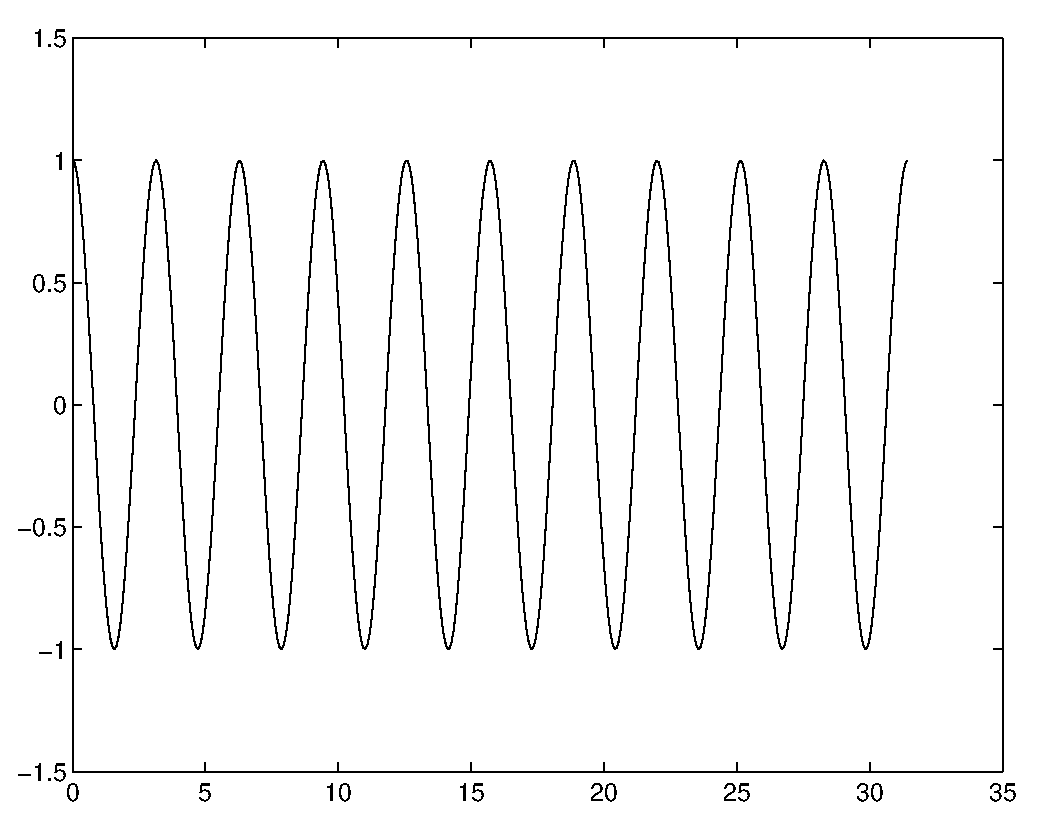
\psfig{file=figures/reson1a.eps,width=3.0in}
           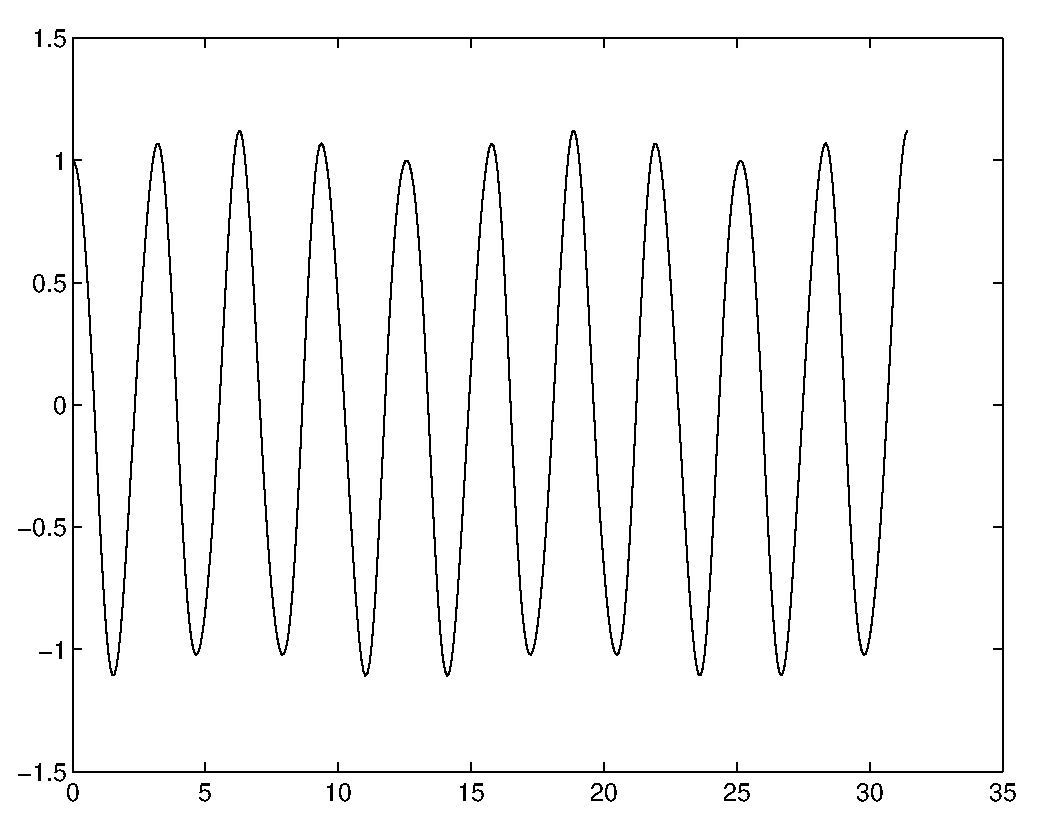
\psfig{file=figures/reson1b.eps,width=3.0in}}
           \caption{Solutions to: (Left) the unforced undamped spring
        equation and (Right) the forced spring equation when $\omega =4.5$.}
           \label{F:nonreson}
\end{figure}

\subsubsection*{Beats}
\index{beats}

Using the trigonometric identity
\[
\cos A - \cos B = -2\sin\left(\frac{A+B}{2}\right)
\sin\left(\frac{A-B}{2}\right),
\]
we find that the solution $x(t)$ is approximately
\begin{equation}  \label{e:x(t)reson3}
x(t) \approx  \frac{1}{1-\omega^2} (\cos(\omega t)-\cos(t))=
\frac{2}{\omega ^2-1}
\sin\left(\frac{\omega+1}{2}t\right)\sin\left(\frac{\omega-1}{2}t\right)
\end{equation}
when $\omega$ is close to $1$.  Note that the first sine term on the right hand
side of \Ref{e:x(t)reson3} has period about $2\pi$ while the second sine term 
has a large period of $4\pi/(\omega-1)$.  For example, when $\omega=1.05$, this
fact leads to periodic behavior of period about $2\pi$ and a 
modulation\index{modulation} 
of period about $80\pi$.  See Figure~\ref{F:beats}.
\begin{figure}[htb]
           \centerline{%
           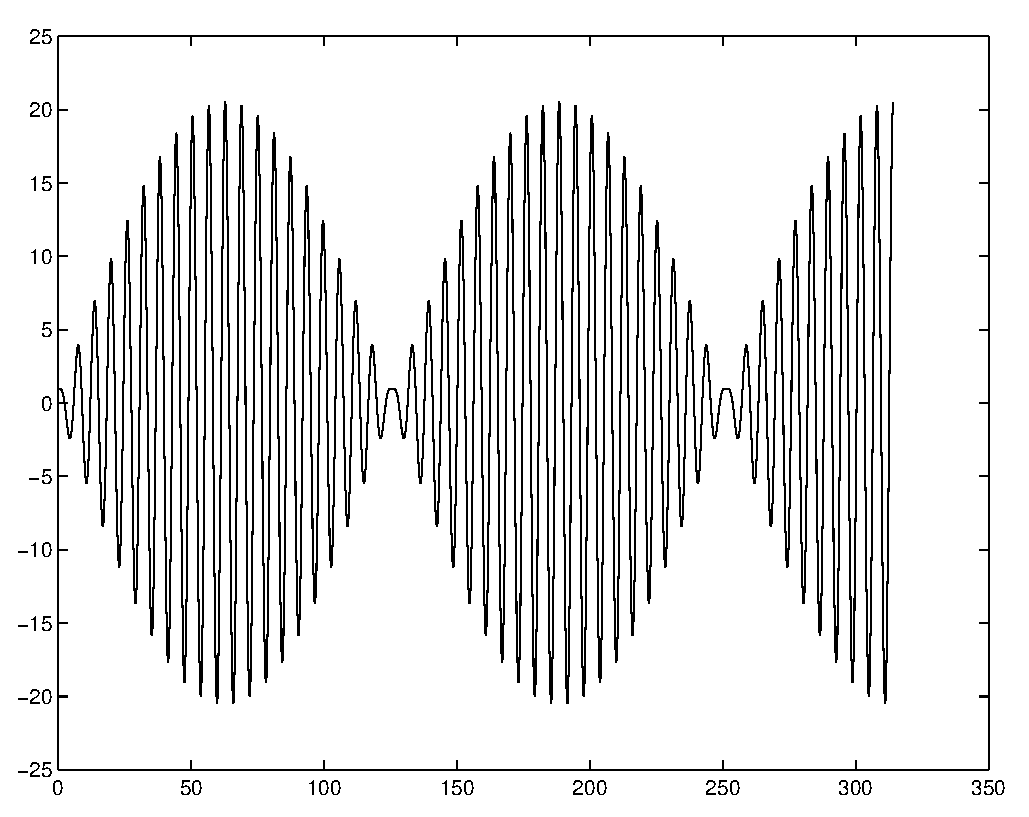
\psfig{file=figures/beats.eps,width=3.5in}}
           \caption{Beats in the solution $x(t)$ to \protect{\Ref{e:x(t)reson}} 
		when $\omega =1.05$ and $0\leq t\leq 100\pi$.}
           \label{F:beats}
\end{figure}  \index{beats}

\subsubsection*{Resonance}
\index{resonance}

When $\omega = 1$ it follows from \Ref{eq:uspfsoln} that every
solution to \Ref{eq:uspf} is unbounded as $t$ goes to infinity.  This
phenomenon is called {\em resonance\/}, and is due to the fact that the
internal frequency\index{frequency!internal} is the same as the 
forcing frequency\index{frequency!forcing}.  The solution
to \Ref{eq:uspf} for $\omega=1$ is shown in Figure~\ref{F:reson} (right).
Resonance shows that when the forcing frequency equals the internal 
frequency, the forcing amplifies the internal dynamics.

Note that when $\omega$ is close to $1$ the solution follows the solution 
for $\omega =1$ for some length of time.  See Figure~\ref{F:reson} where 
the solutions for $\omega =1.05$ and $\omega =1$ are given.  But it is only 
when $\omega =1$ exactly that unbounded growth or resonance actually occurs 
while the nearby solution has long term modulation or beats.
\begin{figure}[htb]
           \centerline{%
           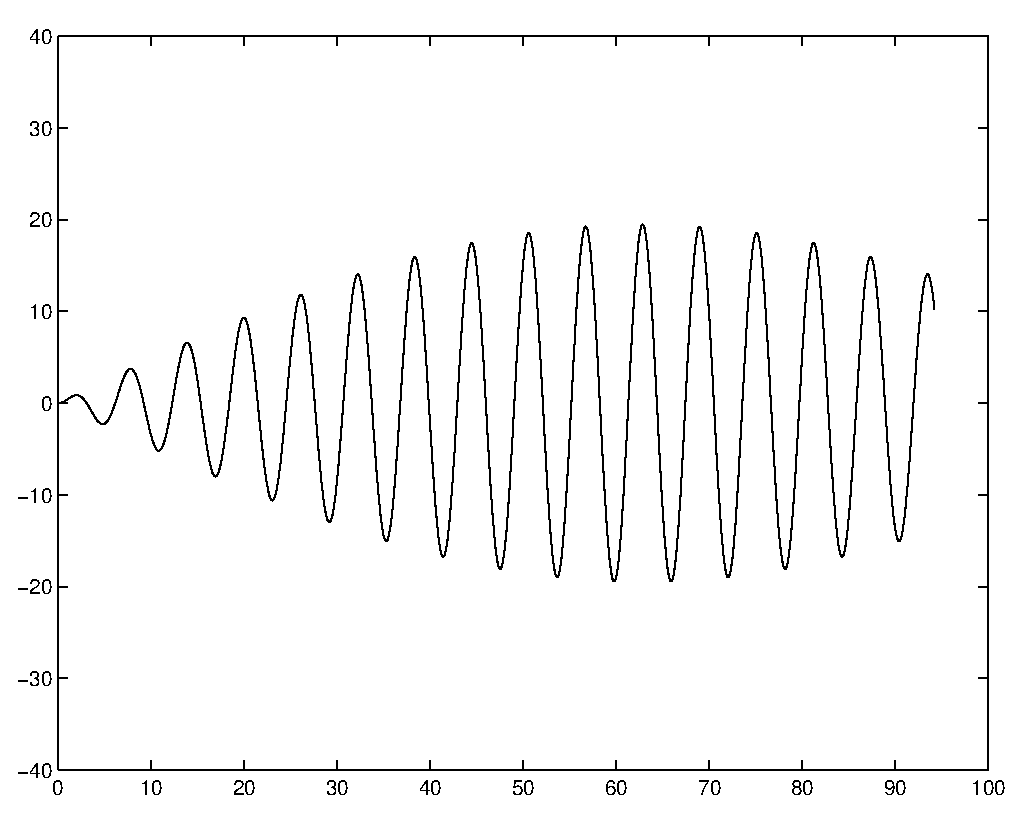
\psfig{file=figures/resona.eps,width=3.5in}
           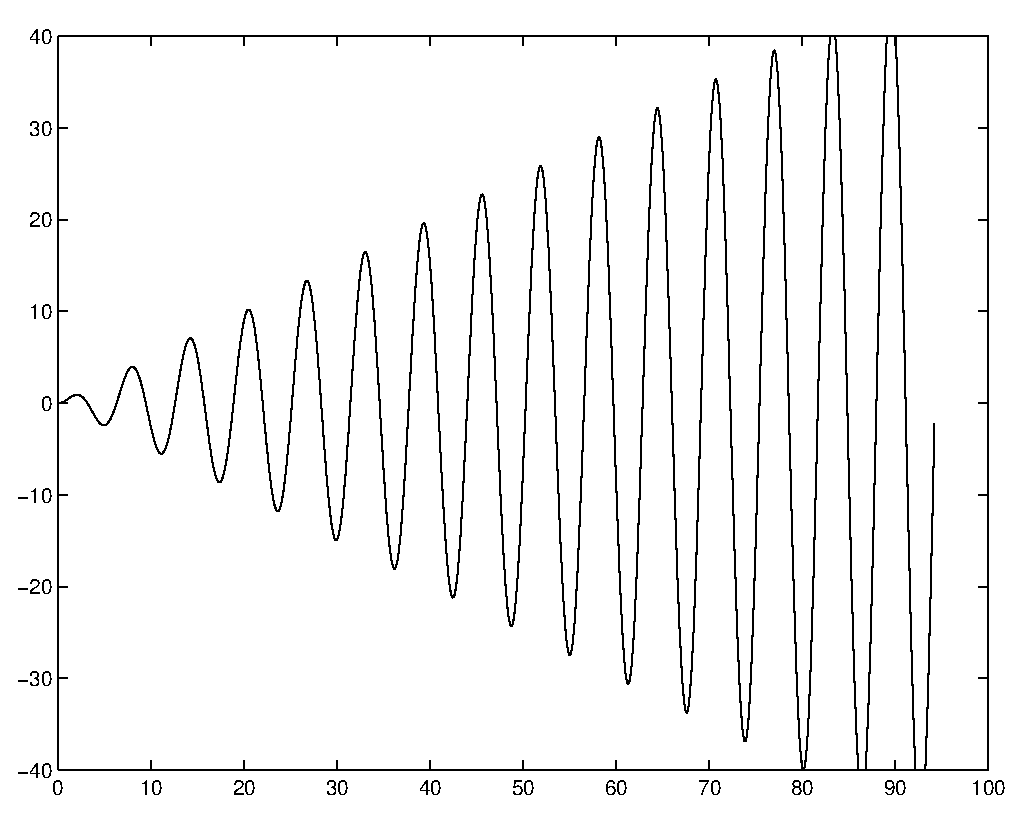
\psfig{file=figures/resonb.eps,width=3.5in}}
           \caption{Two solutions $x(t)$ from \protect{\Ref{e:x(t)reson}} when
                $\omega =1.05$ and $\omega =1$ for $0\leq t\leq 30\pi$.}
           \label{F:reson}
\end{figure}  \index{resonance}



\EXER

\TEXER


\begin{exercise} \label{c12.5.1}
Consider the following equation for the periodically forced
undamped spring\index{spring!undamped!periodically forced}:
\[
\ddot x + \kappa x = A\cos(\omega t).
\]
(Here the constant of the spring $\kappa$ and the amplitude $A$ of the
forcing are assumed to be positive.)  Determine the general solution of
this equation depending on the constants $\kappa$, $A$ and $\omega $.
{\bf Hint:} Proceed as in the text and distinguish between the two
different cases where $\omega \not=\sqrt{\kappa}$ and 
$\omega =\sqrt{\kappa}$.
\end{exercise}

\begin{exercise} \label{c12.5.2}
The following equation describes the behavior of a damped 
spring\index{spring!damped} that is 
forced periodically\index{forcing!periodic}:
\[
\ddot x + 2\dot x + 2x = \sin(2t).
\]
Find real constants $\gamma$ and $\delta$ so that
\[
x_p(t) = \gamma \cos(2t)+ \delta \sin(2t),
\]
is a particular solution of this second order equation.  Write down the
general solution and discuss the behavior of solutions if time $t$
is going to infinity.
\end{exercise}

\begin{exercise} \label{c12.5.3}
Let $x_\omega(t)$ be the solution to \Ref{eq:uspf} given in 
\Ref{e:x(t)reson}.  Show that 
\[
\lim_{\omega\to 1}x_\omega(t) = x_1(t)
\]
for every real number $t$.
\end{exercise} 

\noindent In Exercises~\ref{c12.5.a} -- \ref{c12.5.d} decide whether or not
beats or even resonance occurs in the given differential equations.
\begin{exercise} \label{c12.5.a}
$\ddot{x} + 4x = \cos(2t).$
\end{exercise}
\begin{exercise} \label{c12.5.b}
$\ddot{x} + 16x = \sin(3.9 t).$
\end{exercise}
\begin{exercise} \label{c12.5.c}
$\ddot{x} + 9x = \cos(t).$
\end{exercise}
\begin{exercise} \label{c12.5.d}
$\ddot{x} + 9x = \cos(-3t).$
\end{exercise}

\begin{exercise}  \label{c12.5.4}
Recall the sinusoidally forced second order equation \Ref{eq:uspf}
\[
\ddot x + x = \cos(\omega t).
\]
The second order differential operator that annihilates $\cos(\omega t)$ is
$q(D)=D^2+\omega^2$.  It follows that any solution to \Ref{eq:uspf} must
satisfy the fourth order equation 
\begin{equation} \label{E:ann=res}
q(D)(\ddot x + x)=0.
\end{equation}
Compute the characteristic polynomial of \Ref{E:ann=res} and its roots. Since
the roots typically form two complex conjugate pairs, observe that there is a
connection between the quasiperiodic solutions of this section and those of
Section~\ref{S:NLD}.  What is the special property of these roots that leads
to resonance and why?
\end{exercise}


\end{document}
